\chapter{SYSTEM DESIGN }

 \section{System Architecture}
 Bloomcycle follows a standard Client-Server architecture based on the MVC (Model-View-Controller) design pattern. The React frontend interacts with the Express.js backend via RESTful APIs, which in turn performs CRUD operations on the MongoDB database.

 \section{Database Design}
 The MongoDB database consists of primary collections for secure tracking and personalization.

 \section{UI Design \& Screenshots}
 The user interface of Bloomcycle is designed with a focus on empathy, clarity, and ease of use. It features soft, calming color palettes. The key screens include:

 \subsection{User Authentication}
 New and returning users interact with simple, secure forms to access their cycle data.
 \begin{figure}[H]
     \centering
     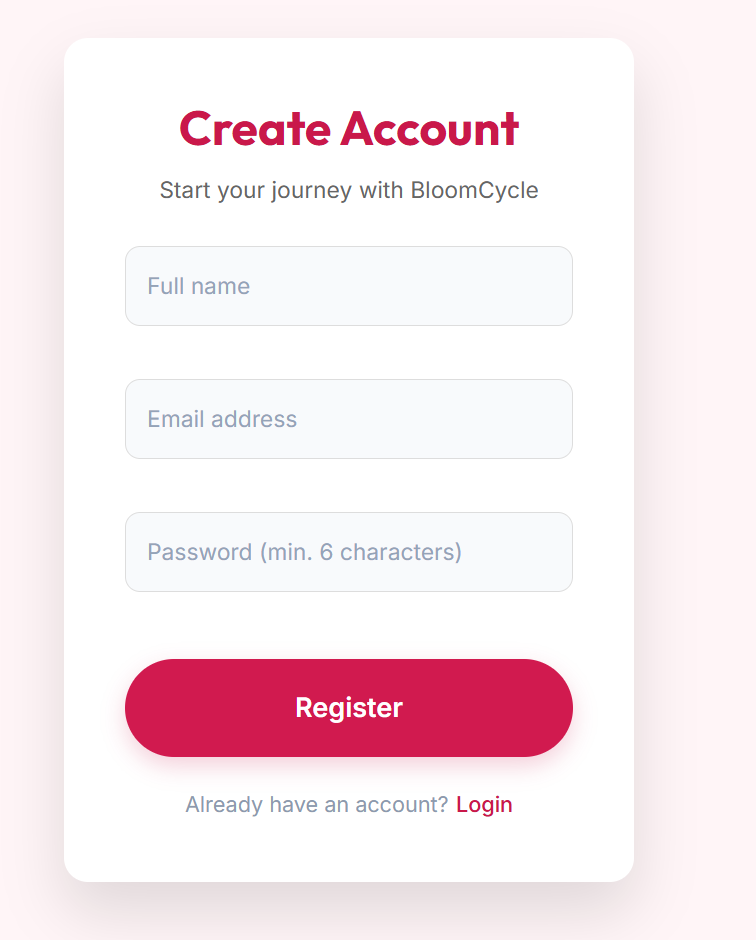
\includegraphics[width=0.8\textwidth]{images/Register.png}
     \caption{User Registration Screen}
 \end{figure}
 \begin{figure}[H]
     \centering
     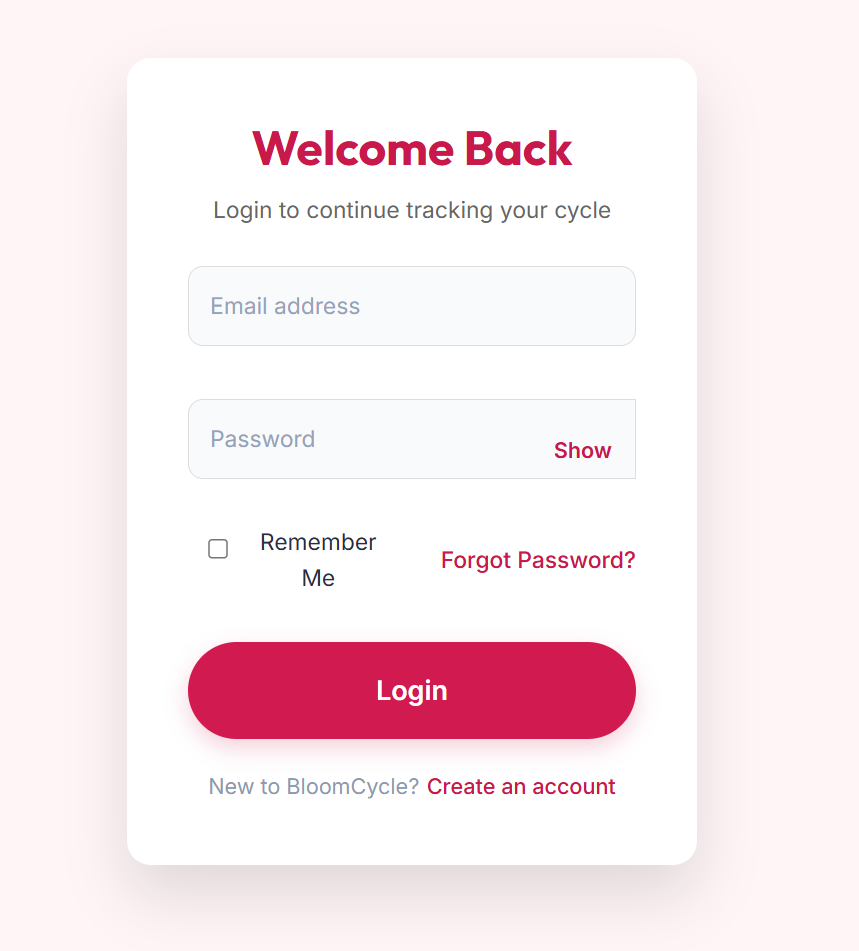
\includegraphics[width=0.8\textwidth]{images/Login.png}
     \caption{User Login Screen}
 \end{figure}

 \subsection{Home \& Features}
 The platform introduces users to its capabilities through an informative landing page.
 \begin{figure}[H]
     \centering
     
\includegraphics[width=0.8\textwidth]{images/Home.png}
     \caption{Application Home Page}
 \end{figure}
 \begin{figure}[H]
     \centering
     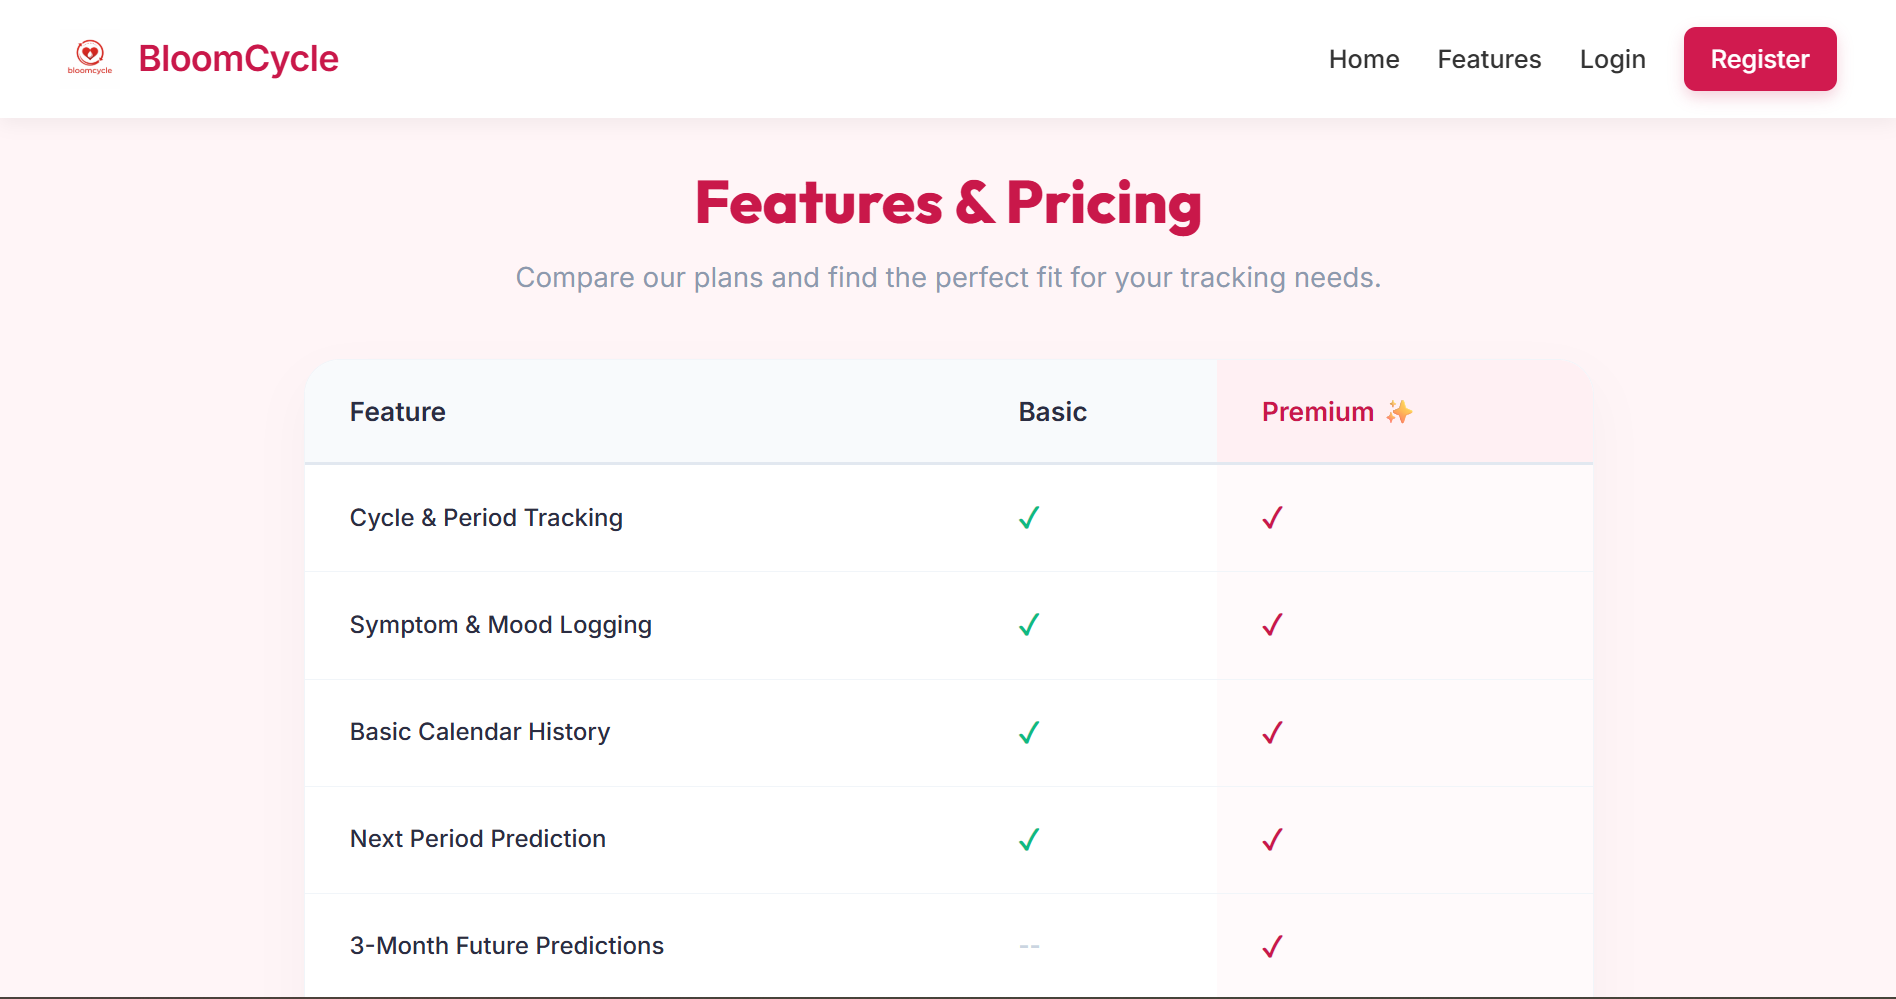
\includegraphics[width=0.8\textwidth]{images/Features.png}
     \caption{Features Overview}
 \end{figure}

 \subsection{Dashboard \& Analytics}
 The main dashboard provides the user with insights into their cycle.
 \begin{figure}[H]
     \centering
     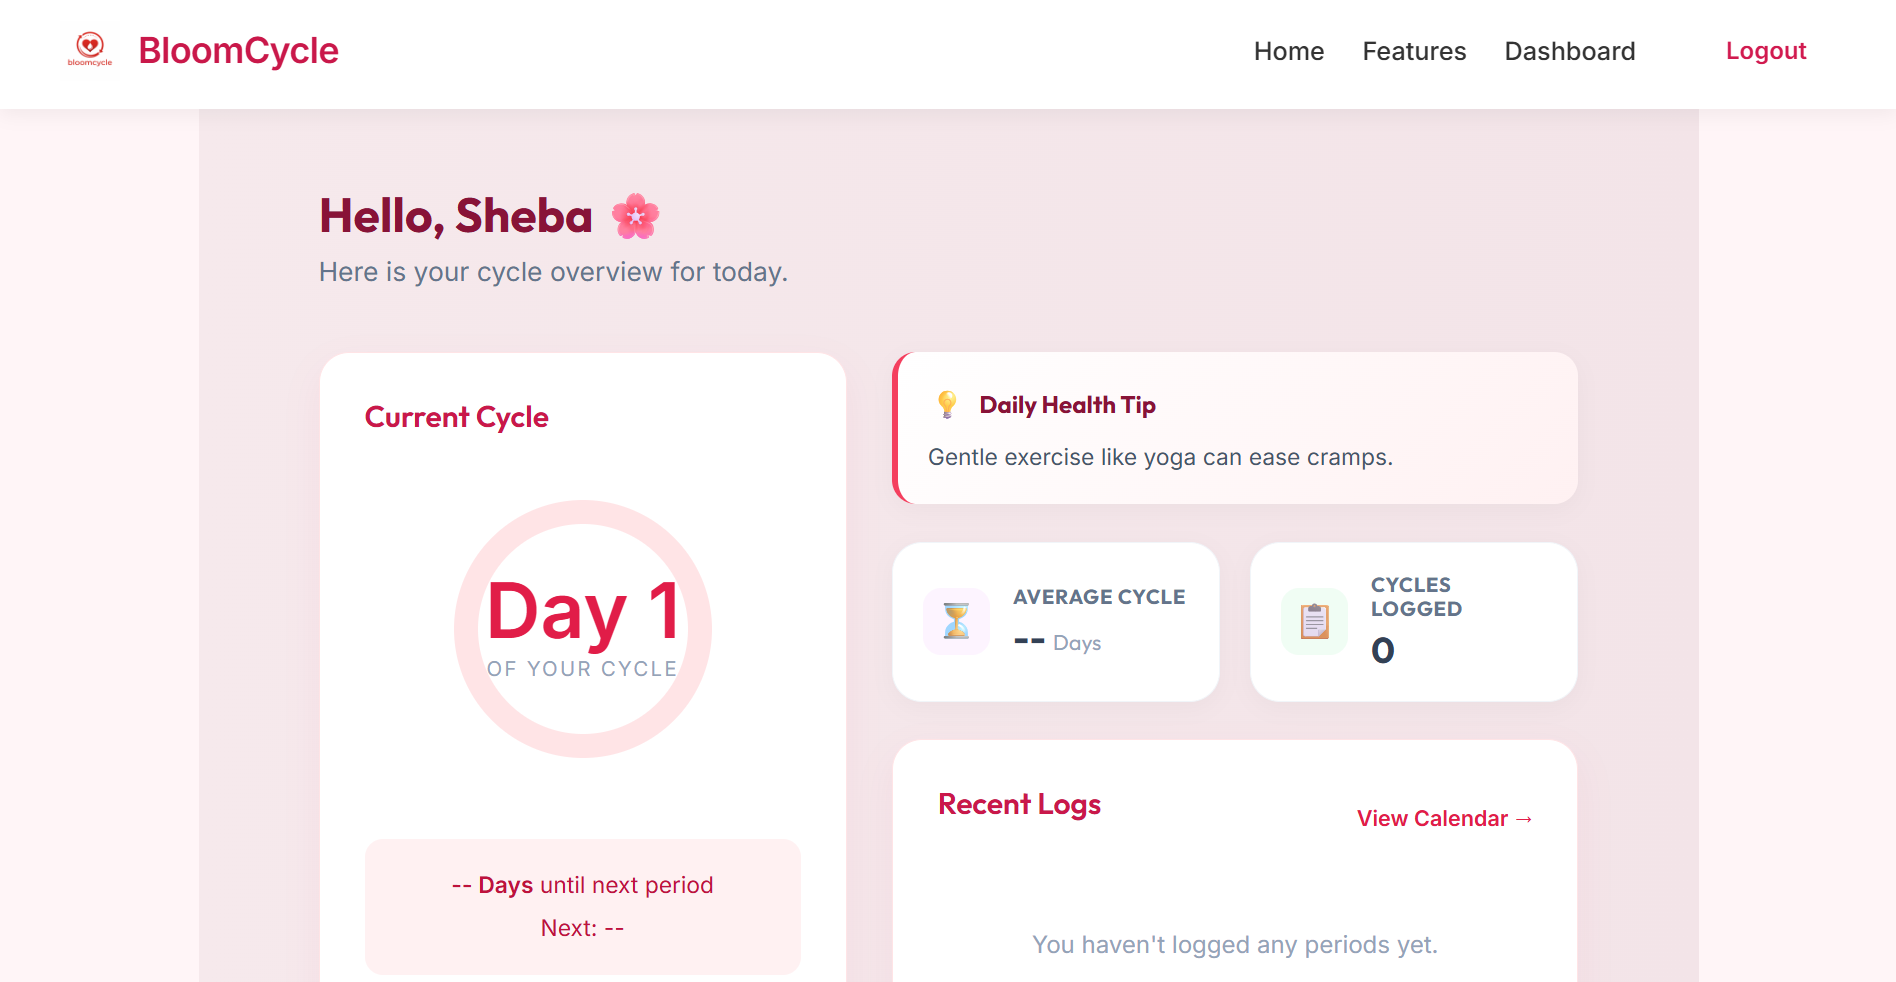
\includegraphics[width=0.8\textwidth]{images/Dashboard.png}
     \caption{User Dashboard}
 \end{figure}

 \subsection{Calendar \& Period Logging}
 Visual grid representations enable users to click on precise dates and view their cycle timeline.
 \begin{figure}[H]
     \centering
     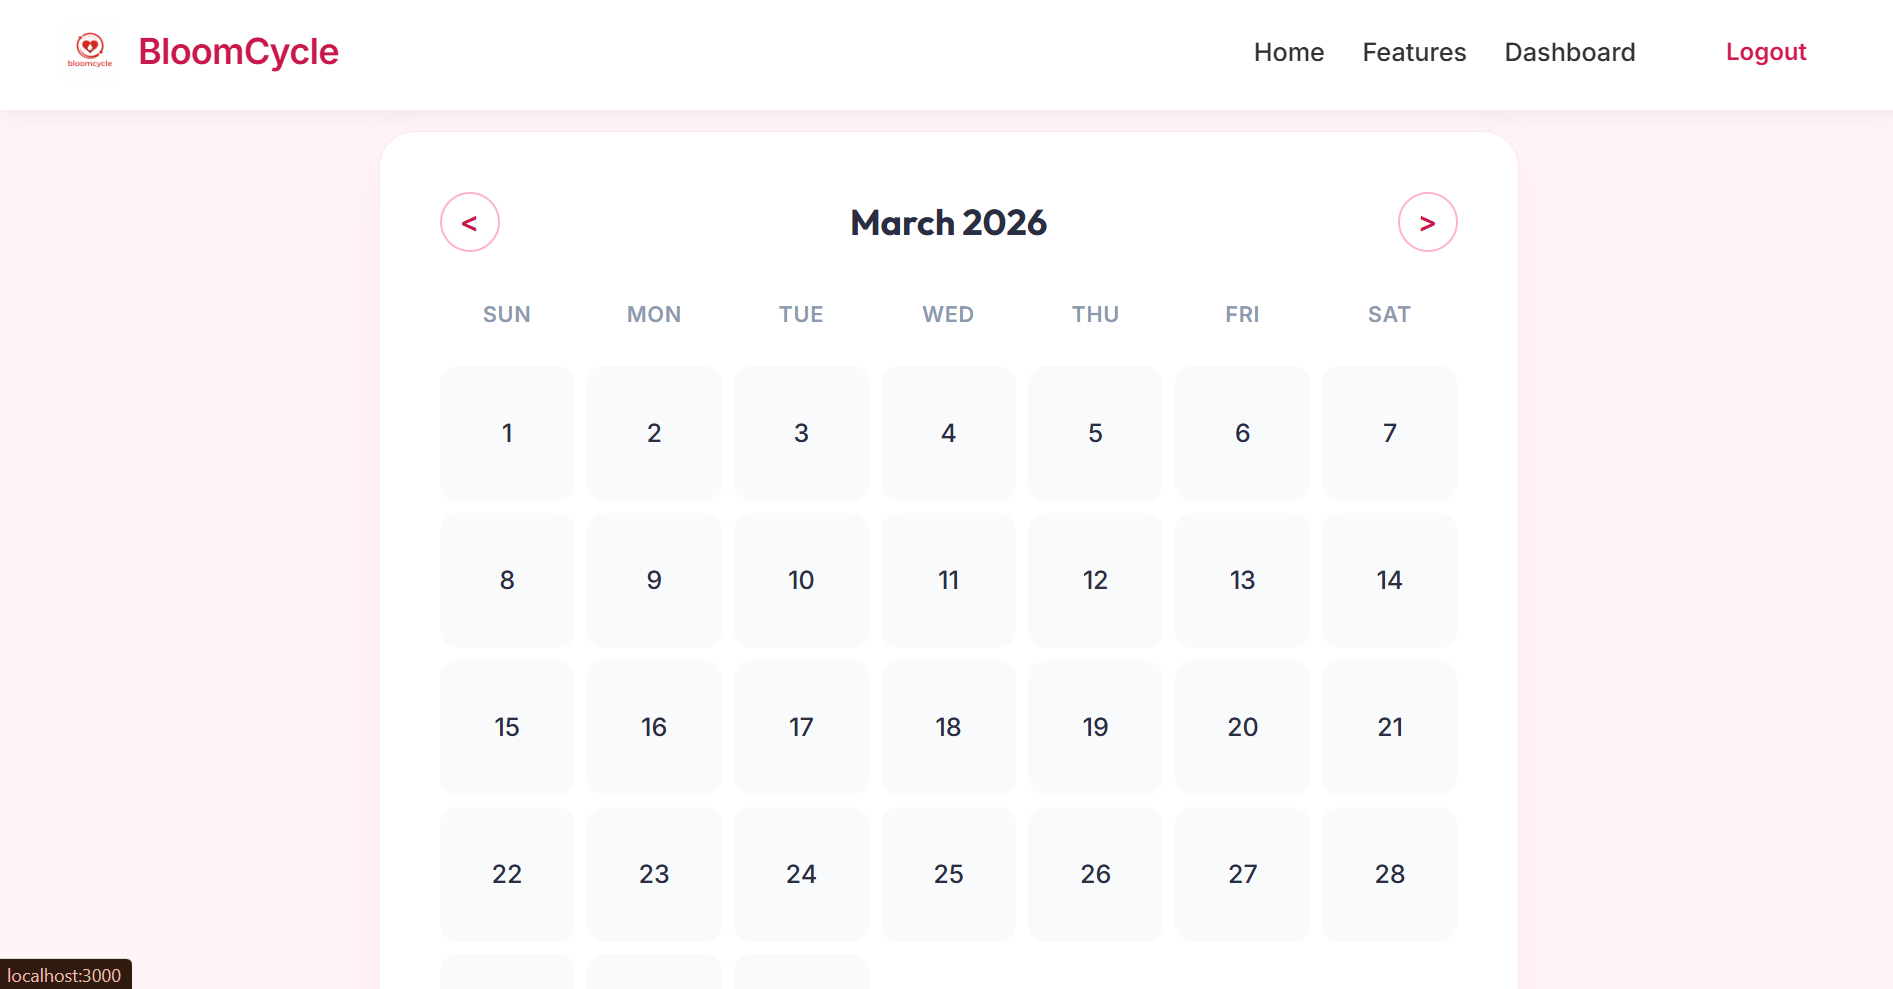
\includegraphics[width=0.8\textwidth]{images/Calender.png}
     \caption{Calendar View}
 \end{figure}
 \begin{figure}[H]
     \centering
     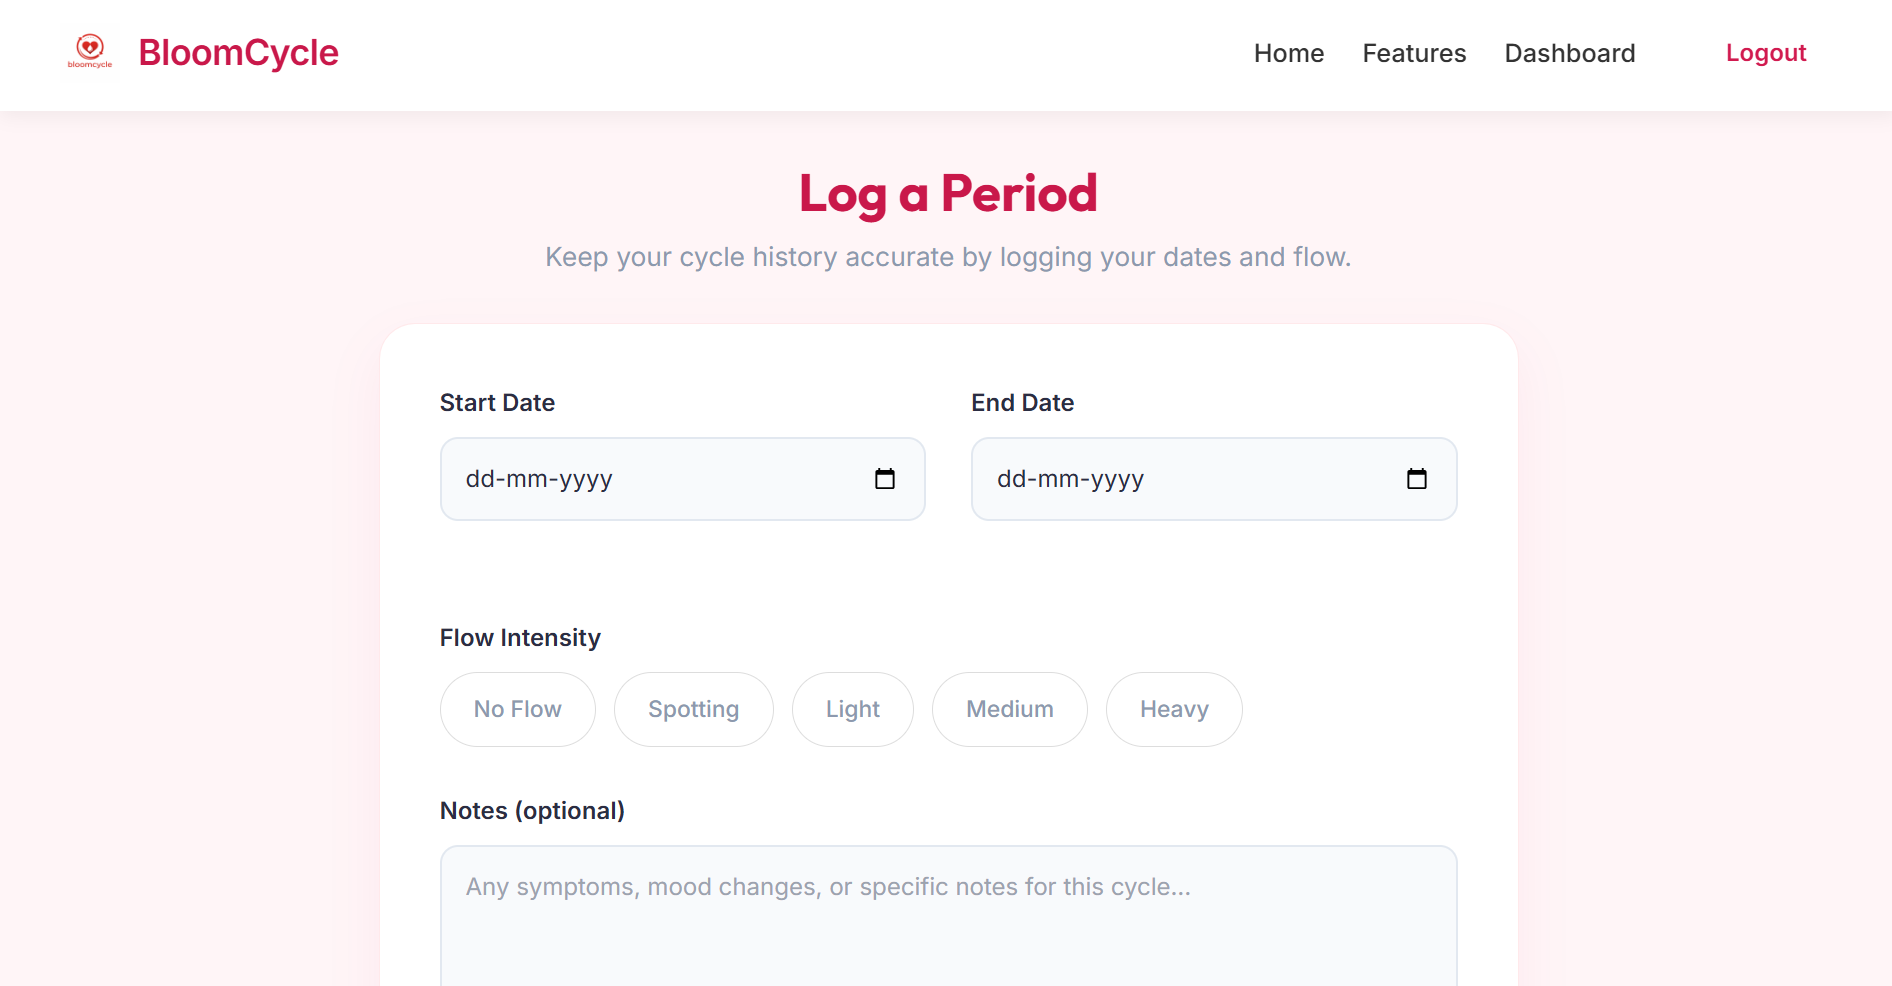
\includegraphics[width=0.8\textwidth]{images/Log_Period.png}
     \caption{Logging a New Period}
 \end{figure}

 \subsection{Symptom Tracking}
 Daily symptom logging allows users to document physical and emotional indicators.
 \begin{figure}[H]
     \centering
     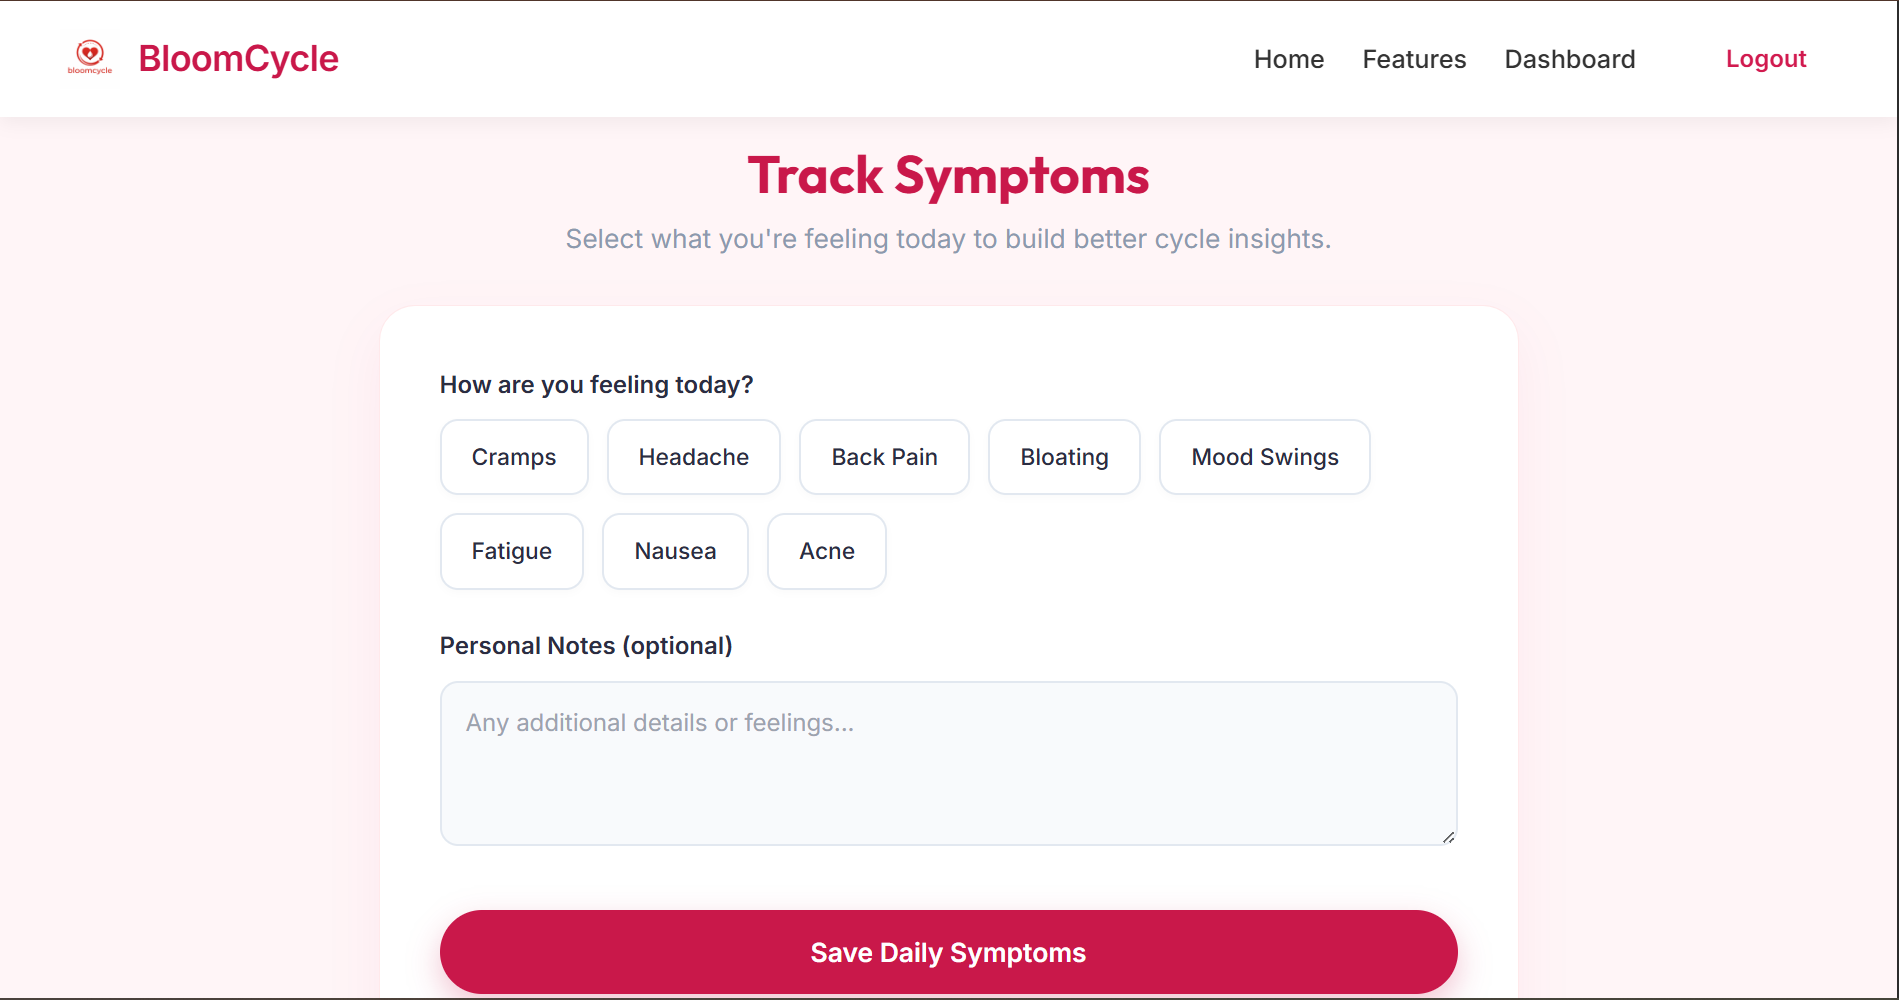
\includegraphics[width=0.8\textwidth]{images/Track Symptoms.png}
     \caption{Track Symptoms Screen}
 \end{figure}

 \section{API Design}
 The backend exposes several secure endpoints:
 \begin{itemize}
     \item \texttt{POST /api/auth/login}: Authenticates a user and returns a token.
     \item \texttt{GET /api/period/insights}: Retrieves historical data based on the authenticated user.
     \item \texttt{POST /api/symptom}: Logs a new symptom for a given date.
 \end{itemize}
